
\section{Research Methodology}\label{sec:method}

This section outlines the research type and its design (cf. Figure \ref{fig:method-overview}), and defines the scope pertaining to identified RQs. We structure our methodology section following the experimental process recommended by Wohlin et al. \cite{wohlin2012experimentation}. Furthermore, we explain and motivate the choice of methods and statistical tests for data analysis. 

We perform an \textit{experiment}, a research method commonly used to explore empirical correlations between several factors, in our case, LLM models and quantization techniques. Given the nature of  experiments, we gain control over subjects, objects, and instrumentation in order to operate on experimental units and draw conclusions on dependent variable output. Experiments are conducted to test the hypotheses and comparatively assess the impact of specific variables in a controlled setting, which is the most suitable setup for answering our RQs.

\begin{figure}[h]
    \centering
    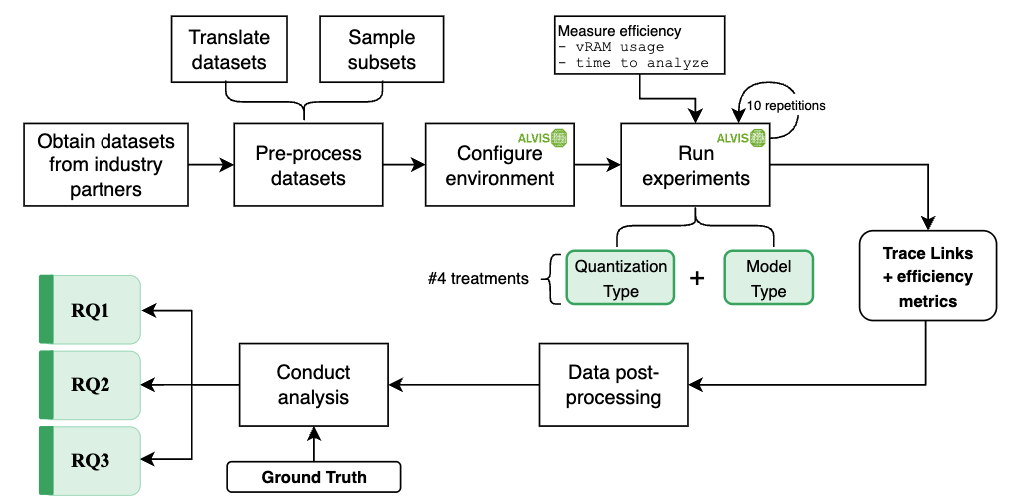
\includegraphics[width=\columnwidth]{images/method-overview-feedback}
    \caption{Overview of the research methodology process}
    \label{fig:method-overview}
\end{figure}

\subsection{Scope and Planning}
We define the scope of our experiment using the said framework of Wohlin et al. \cite{wohlin2012experimentation}. That is, we analyze quantized LLMs for the purpose of evaluation with respect to their efficacy, efficiency, and practicality from the point of view of practitioners in the context of industry REST alignment initiatives.

We conduct a full factorial controlled experiment. There are two factors in our study: baseline models and quantization approaches. We select Mistral as the model factor and three levels for the quantization: \textit{None}, AQW, GPTQ and AQLM.
%There are three levels for the models: LLama, Mistral, and Mixtral; and three levels for the quantization: \textit{None}, GPTQ, \st{GGUF}, AQLM and AWQ. 
% \textcolor{red}{There is sort of only one factor in our experiment... \textit{rewrite the entire design as if we had one factor only}?}


Our model selection is motivated by prior adoption in existing research as well as in industry. Moreover, the Mistral ia an open-weight model, which makes it accessible and transparent in contrast to proprietary alternatives (e.g., ChatGPT). Providers of proprietary LLMs generally do not disclose the internal structure of their models and usage of such models is accompanied by high execution costs. It is also worth noting that the study by Quinstedt and Lindgren \cite{quinstedt2024Optimizing} forms the foundation of our research and their discussion opened up the questions which we explore in our study. Aligning our model selection with theirs allows for a more nuanced and detailed analysis of the trade-offs associated with quantized model versions.

The dependent variables reflect the definition of performance in this study; they are: balanced accuracy, precision, recall, and F1-score (RQ1, efficacy), as well as time-to-analyze and GPU memory-usage (RQ2, efficiency).

Our control variables include a prompt template---used with the REST-at tool in a previous study \cite{quinstedt2024Optimizing}, requirements specification and test case files, as well as mapping files---specifying the correct trace links between tests and requirements. The (ground truth) mappings were derived by employees at reputable industry sources and/or academic researchers. Despite this, there is no guarantee for absolute correctness, however, they are representative of data and standards in both industry and research.

\begin{figure}
    \centering
    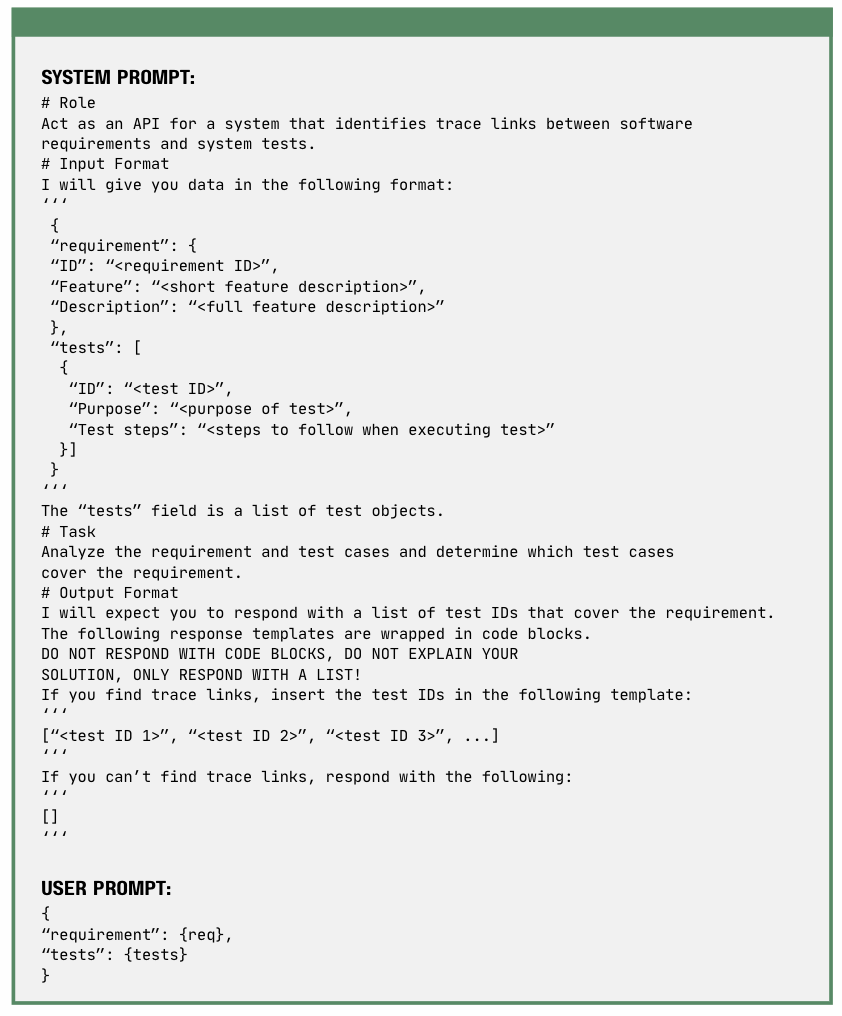
\includegraphics[width=\linewidth]{images/system_prompt}
    \caption{System Prompt Example}
    \label{fig:system_prompt}
\end{figure}

The datasets are as follows: \textbf{AMINA} has been provided to us by our industry partner and originates from G\"oteborg Energi, \textbf{BTHS} was sourced from Bluetooth Headset Profile 1.2\footnote{\url{https://www.bluetooth.com/specifications/specs/headset-profile-1-2/}}. In addition, we have web-scraped a public \textbf{Mozilla} test case repository\footnote{\url{https://www-archive.mozilla.org/quality/browser/front-end/testcases/}} and sourced the \textbf{Health Watcher} requirements document, containing the specification for a public health system, produced through a collaboration between academic and industrial practitioners\footnote{\url{https://zenodo.org/records/8081523}}

We sample the datasets to reduce the overall computational costs in terms of time and to meet resource allocation constraints of the Alvis platform. Requirements are sampled from the full dataset and the connected tests are extracted to create subsets of 25 requirements with varying numbers of tests using Python's built-in PRNG function\footnote{Pseudo-random Number Generator, cf. \url{https://docs.python.org/3/library/random.html}}. 

Furthermore, model hyper-parameters are kept constant and configured consistently across different models. For instance, we set \textit{temperature = 0.1} to control the randomness of the LLM output; a lower value makes the output more deterministic.

% We also standardize the Python environment (version) as it has a direct impact on code execution speeds and therefore also on the benchmarking results. However, the dependency environments have had to be individually adapted for each of the quantization techniques, due to practical reasons, resulting in separate containers for each.

An overview of the experimental design can be found in Figure \ref{fig:exp-design}. See subsection \ref{sec:instrumentation} for further specification of the experiment objects.

%%%%%%%%%%%%%%%%%% HYPOTHESIS TABLE %%%%%%%%%%%%%%%%%%

\newcommand{\equalM}{$M_{1} = \dots = M_{12}$}
\newcommand{\notEqualM}{$M_{1} \neq \dots \neq M_{12}$}

\begin{table}[h]
    \centering
    \caption{Experiment Hypotheses}
    \renewcommand{\arraystretch}{1.65} % original value 1.5
    \begin{tabular}{@{} c p{3.5cm} p{3.5cm} @{}}
    \toprule
    &\multicolumn{1}{c}{\textbf{(i) Efficacy RQ1}}
    &\multicolumn{1}{c}{\textbf{(ii) Efficiency RQ2}} \\
    \midrule
    $H_{0}$ % <-- NULL HYPOTHESIS %
    & There is no difference in \textbf{efficacy} between the treatments
    under test; \equalM.
    & There is no difference in \textbf{efficiency} between the treatments
    under test; \equalM.\\
    $H_{a}$ % <-- ALT HYPOTHESIS %
    & There is a difference in \textbf{efficacy} between the treatments
    under test; \notEqualM.
    & There is a difference in \textbf{efficiency} between the treatments
    under test; \notEqualM.\\
    \bottomrule
    &\multicolumn{2}{c}{Note: the individual treatments are labeled as $M_{1\dots12}$.} \\
    \end{tabular}
    \label{tab:hypothesis}
\end{table}

\subsubsection{Baseline Solution---Cosine Similarity Algorithm}

Previous research on the use of LLMs for REST alignment has not compared their performance against a baseline solution. Therefore, we choose the Cosine Similarity algorithm for this purpose. We apply the following optimization techniques: text preprocessing, stop word removal and TF-IDF vectorization. To accurately assess and compare the performance of this technique with the LLMs, we use the balanced accuracy metric.

\subsection{Data Collection}\label{sec:data-collection}

First, we collect data and derive metrics from repeated test iterations. The process is repeated with 10 repetitions per treatment per dataset (or one repetition per each dataset subset---if they exist, in which case there are ten). We altogether obtain $4 \times 9 \times 10 = 360$ output artifacts, which are result files containing generated trace links and benchmark data. When analyzing the data, we initially examine the treatments from two perspectives: (i) efficacy, and (ii) efficiency---evaluating the null hypotheses for these groups of metrics separately (cf. Table \ref{tab:hypothesis}).

Note that, given the stochastic nature of LLMs, it is important that we perform repeated tests on the same input for each of the treatments in order to include standard deviation measurements across the different metrics; for this reason, we choose to perform 10 repetitions for each treatment. This allows us to reason about the consistency of each treatment as well as increase the validity of our measurements and subsequently the results of our analysis.

Due to the deterministic nature of the Cosine Similarity algorithm, we execute it once on each complete dataset to retrieve the corresponding similarity scores. We calculate the balanced accuracy values using the same formula applied in a confusion matrix.

%%%%%%%%%%%%%%%%%% EXPERIMENTAL DESIGN FIGURE %%%%%%%%%%%%%%%%%%

\begin{figure}[h]
\begin{center}
    \begin{tcbraster}[raster columns=2, raster column skip=5pt, raster equal height=rows, raster row skip=5pt]
        \begin{roundedBox}
            \centering
            \textbf{Independent Variables \& Levels}
            \begin{itemize}
                \item Model:
                \begin{itemize}
                    \item LLama
                    \item Mistral
                    \item Mixtral
                \end{itemize}
                \item Quantization technique:
                \begin{itemize}
                    \item None
                    \item GPTQ Quantization
                    \item AWQ Quantization
                    \item AQLM Quantization
                \end{itemize}
            \end{itemize}
        \end{roundedBox}
        \begin{roundedBox}
            \centering
            \textbf{Objects}
            \begin{itemize}
                \item Hardware (Alvis)
                \item Alvis job-scripts
                \item REST-at tool
                % \item Hardware: local
            \end{itemize}
        \end{roundedBox}
        \begin{roundedBox}
            \centering
            \textbf{Dependent Variables}
            \begin{itemize}
                \item Balanced Accuracy
                \item Precision
                \item Recall
                \item $F1$-score
                \item Time-to-analyze
                \item GPU memory-usage (VRAM)
            \end{itemize}
        \end{roundedBox}
        \begin{roundedBox}
            \centering 
            \textbf{Control Variables}
            \begin{itemize}
                \item Requirements file
                \item Test case file
                \item Ground truth file
                \item Prompt template
                \item Model hyper-parameters
                \item Python environment (version)
            \end{itemize}
        \end{roundedBox}
        \end{tcbraster}
        \begin{roundedBox}
            \centering
            \textbf{Output (artifacts)}
            \begin{itemize}
                \item Result files, containing:
                \begin{itemize}
                    \item Structured trace links
                    \item Benchmark data
                \end{itemize}
            \end{itemize}
        \end{roundedBox}
    \caption{Overview of the experimental design}
    \label{fig:exp-design}
\end{center}
\end{figure}

\subsection{Instrumentation}\label{sec:instrumentation}
For our instrumentation, we extend \verb|REST-at| by adding support for (i) quantized models, and (ii) logging efficiency benchmark data from the models' execution. We run our experiment on Alvis, a cloud platform for scientific computing. The system is built around NVIDIA GPUs, and allows executing jobs on demand. Therefore, we execute the experiments on a dedicated set of available NVIDIA A100 Tensor Core GPUs\footnote{\url{https://www.nvidia.com/en-us/data-center/a100/}}, which inherently makes all performance and efficiency metrics rely on this hardware configuration.

For our experiment, we require a set of requirements linked with a corresponding set of tests. The datasets with trace links serve as \textit{ground truth} since these are established by the authors from the companies.

\subsection{Analysis and Interpretation}\label{sec:analysis}

% FROM METHOD SCOPE - REMOVED
% After testing for our null and alternative hypotheses, we apply a post-hoc pairwise comparative analysis of the treatment pairs. Finally, a descriptive analysis investigates trade-offs of using quantized LLMs for REST alignment; we combine the results from both efficacy and efficiency metrics, as well as some additional factors (e.g., implementation challenges, learning curve) that are described in detail in subsection \ref{sec:analysis}.

The data analysis includes performance indicators from a confusion matrix: balanced accuracy, precision, recall, F1-score. Those measures convey the efficacy of the treatment under test. We use descriptive statistics and data visualization to identify differences between the treatments. 
% derive the mean, median, and standard deviation from the (repeated) tests for each treatment to give reliable measurements for all the different metrics. 

Our full factorial design has two factors. The data is paired as we will be comparing the same data points (rows) between different treatments. First, we will analyze the distribution of the collected data. Specifically, we will use the Shapiro-Wilks test to check for distribution normality and Levene's test to check for homoscedasticity---equal or similar variance between groups. If these tests show that necessary assumptions are met, we will use a parametric two-way ANOVA statistical test. If the assumptions do not hold, we will instead use a non-parametric Friedman test which is an alternative to repeated ANOVA-measures \cite{mccrum2008statisticalTests}.

Should the null hypothesis be rejected, indicating that there is a significant difference between at least one of the treatment pairs, we conduct a pairwise post-hoc analysis to identify the differing pairs as well as in which direction they differ. By evaluating the treatment pairs, we can examine whether certain quantization techniques result in better model performance within the given context. 
%The z-score based Dunn's test will be used for the post-hoc analysis, as the sample size is $>$30 \cite{dunn1964dunnTest}. 
% Can also mention that it is a rank-based follow-up test to Kruskal-Wallis - if we can find a source ... -_-
% ...or the Conover-Iman test \cite{conover1979conoverImanTest} will be used depending on the sample size. 
% NOTE: keeping this here since we might use this test instead (it has better statistical power)? Also, is it okay that we cite the original sources here and not literature that recommends the test's usage?
We use the Holm–Bonferroni method to mitigate \textit{alpha inflation} which would otherwise increase the risk of type I errors---while also reducing the risk of type II errors compared to the regular Bonferroni method \cite{abdi2010HolmBonferroni}.
We will choose between t-test (parametric) or Mann-Whitney (non-parametric), depending on the distribution of the resulting data - BUT when the report is published we will have already made this decision, so this is probably unnecessary to state

% We conduct a descriptive statistical analysis of the results to analyze and discuss the trade-offs of applying quantization to LLMs within the given context.
Ultimately, we are interested in examining whether there exists any treatment(s) that retains acceptable / usable recall and F1-score results despite significantly reducing GPU memory-usage. Thus, we combine the efficacy and efficiency metrics alongside the following additional factors: implementation challenges, learning curve, model VRAM usage compared with commercial GPU alternatives, cost comparison of manual and automatic solutions. 

We choose to represent the data in tables comparing the results from the different treatments. For this purpose, \textit{mean $\pm$ standard deviation} is displayed for each of the relevant metrics. We also select box-plots in order to visualize the distribution as well as any outliers in each treatment's performance. Lastly, we use bar charts to give a clear comparison of the performance as a result of the different quantization techniques.
